\chapter{卖出看涨期权比率}
\section{卖出看涨期权比率}
简单地说,卖出看涨期权比率(ratio call writing)是这样一种策略,投资者持有一定数量的标的股票,同时他卖出了更多股数的看涨期权。因此,卖出的看涨期权所对应的股数与已持有的股数之间就有了一个比率。最常见的比率是 2:1,在这种比率上,投资者持有 100 股标的股票,同时卖出 2 手看涨期权。请注意,这类头寸涉及卖出一定数量的裸期权以及一定数量的备兑期权。由此而产生的头寸,既有卖出备兑看涨期权时的下行风险,又有裸卖出时的无限上行风险。如果标的股票价格在期权存续期内保持相对无变化,卖出看涨期权比率的盈利会比只卖出备兑看涨期权和只卖出裸看涨期权都要大得多。不过与卖出备兑看涨期权和裸看涨期权不一样,卖出看涨期权比率在两个方向上都面临风险。

一般而言,某个投资者在建立卖出看涨期权比率头寸的时候,他应当对标的股票的前景保持中立。这就是说,他卖出的是行权价最接近当前股票价格的看涨期权。
\begin{figure}
    \centering
    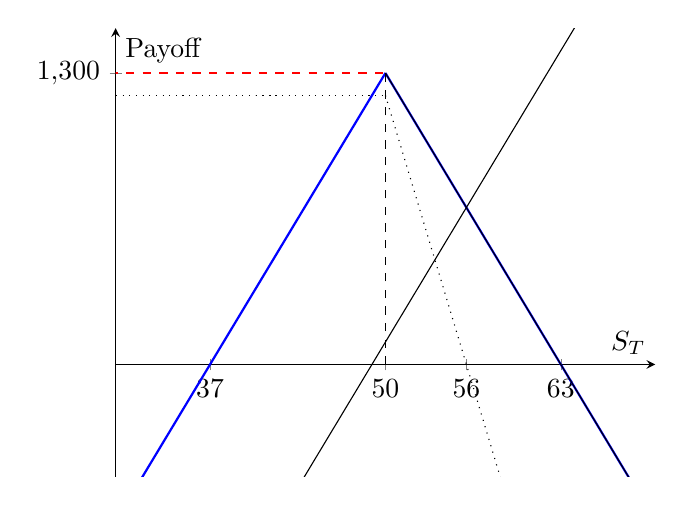
\begin{tikzpicture}
        \begin{axis}[
                axis lines=middle,
                xlabel={$S_T$},
                ylabel={Payoff},
                xmin=30, xmax=70,   % 调整x轴的范围
                ymin=-500, ymax=1500, % 调整y轴的范围
                xtick={37,50,56,63},
                ytick={1300},
                domain=0:100, % 调整绘制曲线的 x 轴范围
                samples=100,
            ]
            % 设置期权参数
            \pgfmathsetmacro\K{50} % 执行价格
            \pgfmathsetmacro\multiplier{100} % 合约乘数

            % 画看涨期权到期收益线
            \addplot[thick,blue,domain=0:50] {(x-37) * \multiplier};
            \addplot[thick,blue,domain=50:100] {(63-x) * \multiplier};
            \addplot[domain=50:100] {(63-x) * \multiplier};
            \addplot[] {(x-49) * \multiplier};
            \addplot[domain=0:\K,dotted] {2 * 6 * \multiplier};
            \addplot[domain=\K:100,dotted] {2 * (56-x) * \multiplier};

            % 在执行价格标注
            \draw[thick,red,dashed] (axis cs:0,1300) -- (axis cs:\K,1300);
            \draw[dashed] (axis cs:\K,0) -- (axis cs:\K,1300);
        \end{axis}
    \end{tikzpicture}
    \caption{期权到期收益图:通过按 49 买入 100 股 XYZ 股票,同时按每手 6 点卖出 2 手 XYZ 10 月 50 看涨期权来建立一个卖出看涨期权比率头寸。}
\end{figure}